\section{Apéndices}

	\subsection{Apéndice A: Enunciado}
		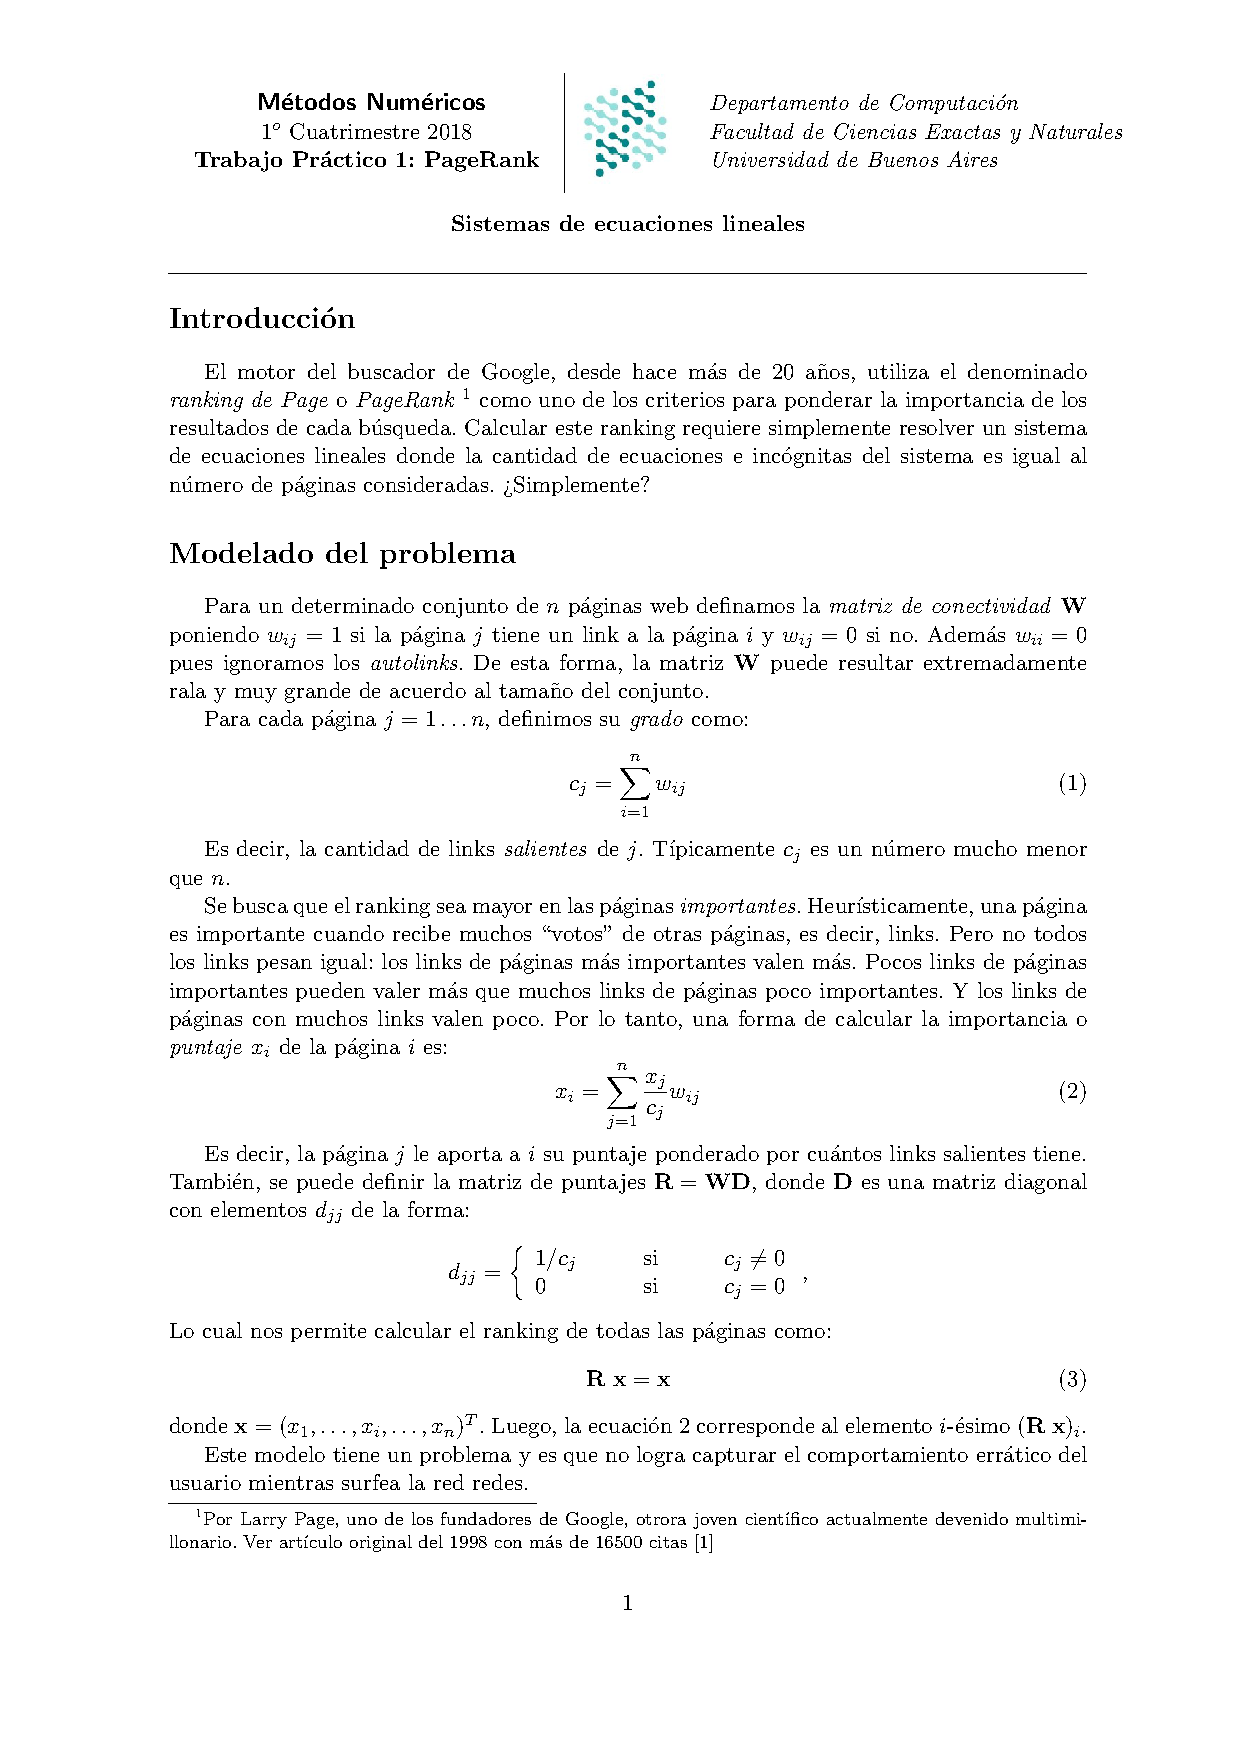
\includepdf{../Enunciado_TP1.pdf}
	%\clearpage

	\subsection{Apéndice B: Código fuente numericamente relevante}
	\clearpage

		\subsubsection{\textit{Page Rank}}

			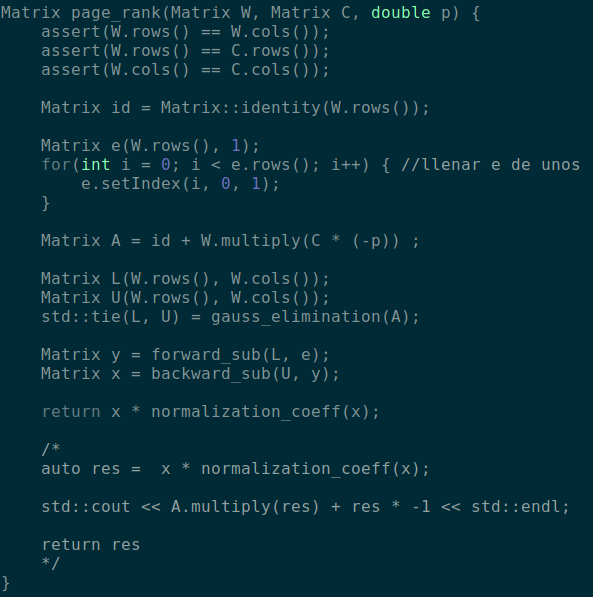
\includegraphics[scale=0.75]{img/src/page_rank}


		\subsubsection{Eliminación Gaussiana}

			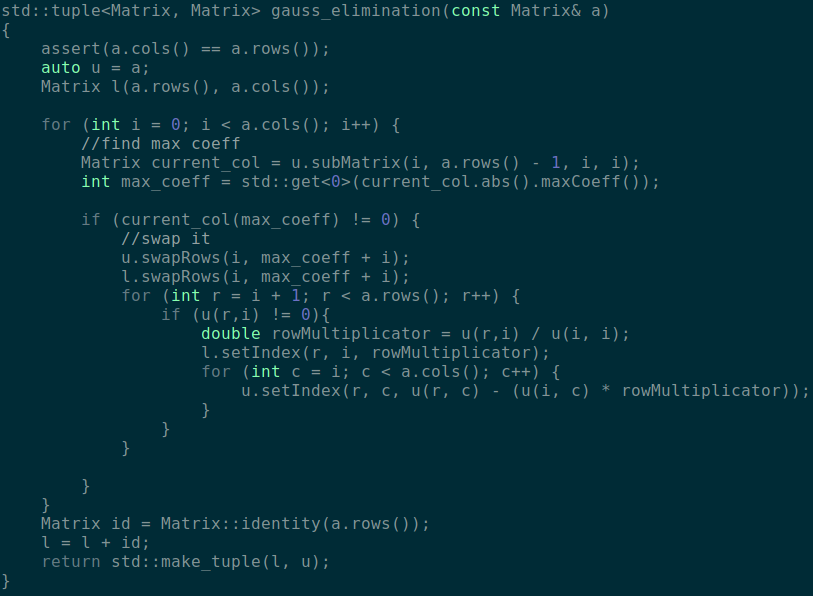
\includegraphics[scale=0.6]{img/src/gaussian_elimination}


		\subsubsection{\textit{Backwards Substitution}}

			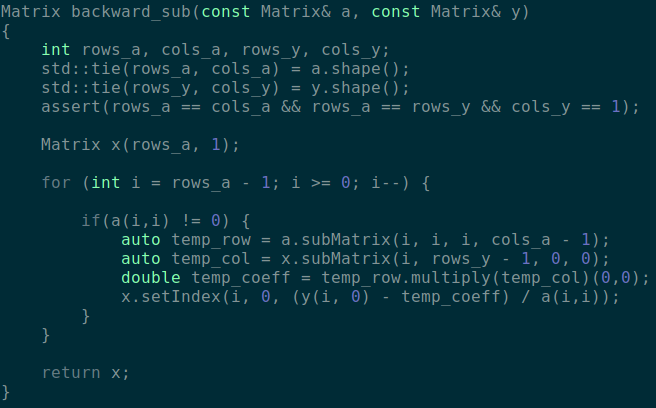
\includegraphics[scale=0.75]{img/src/backwards_substitution}


		\subsubsection{\textit{Forward Substitution}}

			No lo incluímos por ser análogo a backwards substitution. \\


	\subsection{Apéndice C: Demostración $A = pWD + ez^{t}$}

		Se quiere ver que $A = pWD + e z^{t}$ \\

		Vamos a demostrar la igualdad para $1 \leq i \leq n$ y $1 \leq j \leq n$. \\

		\[ \text{Sea $A \in \mathbb{R}^{nxn} /$ } a_{ij} =
		        \begin{cases}
		                (1-p)/n + (p \, w_{ij})         & \text{si } c_{j}  \neq 0 \\
		                1    /n                         & \text{si } c_{j}   =   0
		        \end{cases}
		\]

		\[ \text{y sea $D \in \mathbb{R}^{nxn}$ una matriz diagonal $/$ } d_{ij} =
		        \begin{cases}
		                1/c_j         & \text{si } c_{j}  \neq 0 \\
		                1/n           & \text{si } c_{j}   =   0
		        \end{cases}
		\]

		Como multiplicar por derecha por una matriz diagonal (en este caso $D$), es multiplicar a cada columna de $W$ por elementos de la diagonal de $D$, entonces: \\

		\[ (pWD)_{ij} =
		        \begin{cases}
		                (p \, w_{ij})/c_j 	& \text{si } c_{j}  \neq 0 \\
		                0 			& \text{si } c_{j}   =   0
		        \end{cases}
		\]

		Notar que $p$ es un escalar, y la operación $WD$ se puede hacer porque ambas matrices pertenecen a $\mathbb{R}^{nxn}$ (ver las definiciones de las matrices en la introducción teórica o en el enunciado del trabajo práctico). \\

		\[ \text{Sean }
		        e       = \begin{pmatrix}
		                        1 \\
		                        \vdots \\
		                        1
		                \end  {pmatrix}
		\qquad
			\text{ y }
		\qquad
			z_{j} = \begin{cases}
		                        (1-p)/n & \text{si } c_{j} \neq 0 \\
		                         1   /n & \text{si } c_{j}   =  0
				\end  {cases}
		\]

		Entonces $e z^{t}$ es una matriz en $\mathbb{R}^{nxn}$, con $z^{t}$ en cada fila: \\

		\[
		        e z^{t} 	= 	\begin{pmatrix}
							1 \\
							\vdots \\
							1
						\end  {pmatrix}
						\begin{matrix}
							\begin{pmatrix}z_1 & \hdots & z_n
							\end  {pmatrix}\\\mbox{}
						\end{matrix}
					= 	\begin{pmatrix}
							z^t 	\\
							z^t 	\\
							\vdots 	\\
							z^t
						\end  {pmatrix}
		\]

		\[
			        ez^{t} = \begin{cases}
						(1-p)/n & \text{si } c_{j} \neq 0 \\
						 1   /n & \text{si } c_{j}   =  0
					 \end  {cases}
		\]

		Entonces $pWD \in \mathbb{R}^{n}$ y $ez^{t} \in \mathbb{R}^{nxn} =>$ se pueden sumar. \\

		Los valores de ambas dependen de $c_j => pWD+ez^t$ queda definida como:

		\[
			        pWD+ez^{t} = 	\begin{cases}
							pw_{ij}/c_j+(1-p)/n & \text{si } c_{j} \neq 0 \\
								     1   /n & \text{si } c_{j}   =  0
						\end  {cases}
		\]

		Por conmutatividad de la suma en el caso $c_j \neq 0$ podemos ver que se trata efectivamente de la matriz $A$. \\

		\qed

	\clearpage

	\subsection{Apéndice D: Aplicabilidad E.G., condicionamiento de la matriz $(I-pWD)$ e influencia del valor $p$ en ello}

		La E.G. se aplica sobre el \textit{ranking} de Page: \\

		El \textit{Page Rank} es la solución al sistema $Ax=x$. La matriz $A$ puede reescribirse como $A=pWD+ez^{z}$ por lo visto en el apéndice C. Sean la matriz $D$ y los vectores columna $e$ y $z$. \\

		\begin{equation}
			Ax=x \Leftrightarrow 0 = x-Ax \Leftrightarrow 0 = (I-A)x \Leftrightarrow 0 = [I - (pWD+ez^{t})]x \Leftrightarrow ez^{t}x = (I-pWD)x
		\end{equation}

		Suponemos $z^{t}x = 1 => (I-pWD)x = e$. \\

		Sabemos por el teorema 6.21 del Burden $[0]$, que si $A$ es estrictamente diagonal dominante por columnas (EDDc), entonces tiene factorización LU. \\ %Acá va una cita %TODO

		Se quiere ver que $A$ es EDDc para garantizar la aplicabilidad de la eliminación gaussiana, es decir que: \\

		\begin{equation}
			|a_{jj}| > \sum^{n}_{i=1, i \neq j} |a_{ij}| \text{para} j = 1, \hdots, n
		\end{equation}

		Es decir, que la suma en módulo de los elementos de la columna (excepto del elemento en la diagonal), es menor al módulo del elemento de la diagonal correspondiente a esa columna. \\

		\begin{equation}
			|a_{jj}| = a_{jj} = 1 \forall j = 1, \hdots, n
		\end{equation}

		Pues $(-pWD)_{jj} = 0$ y $I_{jj} = 1, \forall j$, entonces $(-pWD + I)_{jj} = a_{jj} = 0 + 1 = 1$ \\

		Entonces tenemos: \\

		\begin{equation}
			|a_{jj}| = 1 > \sum_{i=1, i \neq j}^{n} |a_{ij}|, \forall j = 1, \hdots, n
		\end{equation}

		Como la sumatoria de la desigualdad de arriba excluye explicitamente a los elementos de la diagonal, podemos no considerar a la matriz diagonal $I$ como parte de ella. \\

		Por otro lado, por ser una sumatoria de módulos, podemos desestimar el signo negativo. También, por no depender de la sumatoria, podemos sacar a la $p$ fuera de ella. Entonces: \\

		\begin{equation}
			\sum_{i=1, i \neq j}^{n} |a_{ij}| = \sum_{i=1, i \neq j}^{n} |I-pWD| = p \sum_{i=1, i \neq j}^{n} WD
		\end{equation}

		Notar que $w_{i,j} \geq 0 \forall i,j = 1, \hdots, n$ y $d_{ij} \geq 0 \forall i,j = 1, \hdots, n$. \\

		Entonces $(WD)_{ij} \geq 0 \forall i,j = 1, \hdots, n$. Por eso es posible desestimar el módulo. \\

		$WD$ consiste en multiplicar $col_{j}(W)$ por $d_{jj}$. \\

		Por definición de $D$, si $c_{j} = 0$, entonces $d_{jj} = 0$ por lo tanto $p \sum_{i=1, i \neq j}^{n} WD = 0 < 1$. \\

		Si $c_{j} \neq 0 => d_{jj} = \frac{1}{c_{j}}$. Además $c_{j} = \sum_{i=1}^{n} w_{ij}$. Entonces:\\

		\begin{equation}
			p \sum_{i=1, i \neq j}^{n} (WD)_{j} = p \sum_{i=1, i \neq j}^{n} (w \frac{1}{c_{j}})_{j} =
			p \sum_{i=1, i \neq j}^{n} w_{ij} \frac{1}{c_j} = p \sum_{i=1, i \neq j}^{n} \frac{1}{\sum_{i=1}^{n} w_{ij}} =
			p 1 = p
		\end{equation}

		y por definición $0 \leq p \leq 1 \text{(por ser una probabilidad)} \therefore \sum_{i=1, i \neq j}^{n} |I-pWD| < 1$ \\

		Gracias a esto, puedo asegurar que la suma de los módulos de los elementos de cada columna de la matriz, es menor estricta al elemento de la diagonal para el peor caso (todos los elementos de la columna de $W$ iguales a $1$) y por lo tanto, para cualquier caso. \\

		Por lo tanto, $A$ es estrictamente diagonal dominante por columnas, entonces tiene factorización $LU$ y se puede aplicar el algoritmo de eliminación gaussiana (sin pivoteo o naíf). \\

		\qed

	\clearpage

